\vspace{1cm}

\itshape
En este capítulo se lleva a cabo un estudio de la confiabilidad de tres tipos
de topologías tolerantes a fallas (Sección \ref{seccion:TopologiaEstudio}
página \pageref{seccion:TopologiaEstudio}), candidatas a ser utilizada en el
diseño de la arquitectura propuesta en este trabajo de tesis.

Para ello, en la Sección \ref{sec:req_analisis} (página \pageref{sec:req_analisis})
se realiza una descripción de algunos requerimientos (no estrictos), que guiarán
el desarrollo de una arquitectura para un misión satelital ficticia basada en
componentes COTS. En base a estos ``requerimientos'', se presentan los modelos para
la medición de confiabilidad de las topologías mencionadas en el párrafo anterior. 

En la Sección \ref{sec:protocolo_communicacion} (página \pageref{sec:protocolo_communicacion})
se describe resumídamente el protocolo CANae 0.1 Alpha, que está basado en CAN y
que fue desarrollado en este trabajo de tesis. En el apéndice \ref{Appendix:A}
se describe este protocolo con mayor detalle
\upshape

\noindent\rule{\textwidth}{2pt}

\vspace{1cm}
% section that make an introduction
%\chapter{Introducción}\label{chap:intro}
% TODO: Introuducción, extraída desde el plan de tesis,
En el marco del Plan Espacial Nacional, desarrollado por la \ac{CONAE} de Argentina, y con el propósito de llevar a cabo actividades de investigación y 
aplicación, provenientes de la \ac{UNLAM} se presenta este plan de tesis con el fin de ampliar los 
conocimientos y la participación de la \ac{CONAE} y \ac{UNLAM}, en el campo del Desarrollo Informático y 
Ciencias de la Computación.

Las actividades desarrolladas para este trabajo de tesis son realizadas, en su mayor proporción, en 
la Unidad de Desarrollo \ac{INVAP}, ubicada en San Carlos de Bariloche, Provincia de Río Negro. Este 
trabajo se encuentra orientado a brindar un nuevo conocimiento, que ayude en cierta medida, en el 
desarrollo de los diferentes proyectos con los que cuenta actualmente esta empresa, agregando un 
grado de innovación en el resultado que se obtenga.

\ac{INVAP} tiene como visión ser un referente en proyectos tecnológicos a nivel mundial \cite{invapWEB}, 
por lo tanto, debe asegurarse que cada uno de los productos que se lleven a cabo sean competitivos. 
Para lograr cumplir con esto, es necesario que tales proyectos se encuentren a la vanguardia 
tecnológica y científica.  

El desarrollo de proyectos satelitales conlleva costos de importante magnitud, y 
dependen de cada misión. Una parte importante de los costos está conformado por el 
desarrollo\footnote{\textit{Nota: entiéndase por desarrollo al proceso de planificación, análisis, 
diseño e implementación.}} y sobre todo los materiales que se utilizan para su fabricación. Esto 
es debido a que se utilizan componentes que son exclusivos para el ámbito espacial, en otras 
palabras que se encuentran ``calificados para volar''. Estos componentes son fabricados especialmente para soportar el ambiente hostil del espacio.

Si se considera al ámbito espacial como una industria, algo que ha sido demostrado en los últimos 
años; y si se tiene en cuenta las intenciones de crecimiento y competitividad de la empresa INVAP,  de permitir el ingreso de nuestro pais en el mercado satelital \cite{invapWEB}, resulta de gran 
importancia lograr reducir los costos en fabricación y desarrollo de vehículos satelitales.

La \ac{NASA} tiene un enfoque de desarrollo bajo el lema 
``faster, cheaper, better'' \cite{Forsberg99}, lo cual busca desarrollar sus proyectos y misiones 
de foma rápida, barata y mejor. Bajo este enfoque se han realizado diversos estudios e 
investigaciones dando resultados sumamente positivos \cite{Tai99}, \cite{Chau99}, 
\cite{Schneidewind98}, \cite{Forsberg99}. En estos trabajos se utilizan componentes que no se 
encuentran ``calificados para volar'',  los cuales también son llamados componentes \ac{COTS}, o de estantería. Debe mencionarse, que también hubo algunos 
fracasos en su aplicación. 

A simple vista, la utilización de estos componentes ayudaría a reducir costos. Sin embargo, esto 
no es tan directo. Los componentes \ac{COTS} al no estar calificados, se les deben realizar tareas 
de calificación adicional. Además deben ser aplicados a un ambiente, que asegure 
que no fallarán durante la misión; o si fallan, no será motivo de pérdida de la misma. 

Los componentes \ac{COTS} suelen tener un costo de compra entre 100 y 1000 veces menores que aquellos 
que está califcados para volar. Por lo que el aumento en la utilización de estos componentes, 
aplicados al desarrollo de diferentes tipos de satélite, \textbf{permitiría reducir los costos y 
ahorrar algunos millones de dólares del proyecto satelital.} Esto facilitaría el ingreso de 
Argentina en un mercado altamente competitivo.

El desafío de este trabajo de tesis es analizar y estudiar arquitecturas que sean tolerantes a 
fallas, que permitan una correcta comunicación entre los diferentes subsistemas de un vehículo 
espacial de nueva generación, y que tenga como característica principal un cierto grado de confiabilidad, de modo tal que pueda ser aplicado con componentes \ac{COTS}.

\section{Motivación}\label{chap:motivacion}
Los costos de un proyecto satelital se pueden clasificar, a grandes rasgos, en 5 grupos:
\begin{itemize}
 \item Desarrollo
 \item Materiales
 \item Ensamblado, integración, y tests
 \item Lanzamiento
 \item Operaciones
\end{itemize}

Este trabajo de tesis se centrará principalmente en el desarrollo (proceso de planificación, 
análisis, diseño e implementación.), y en los materiales utilizados en la fabricación de vehículos satelitales.

No se puede mencionar a ciencia cierta cuál es el costo “verdadero” de desarrollar un satélite. Este 
depende exclusivamente del tipo de satélite y de la misión. Lo que si se debe tener en claro es que 
las tareas de desarrollo representan una parte muy importante del costo total del proyecto.

Desarrollar un vehículo espacial con componente \ac{COTS}, en un principio podría representar costos 
adicionales, ya que se le deben realizar tareas de calificación adicional, debido a que no están 
“preparados” para resistir las condiciones hostiles del espacio. 

Uno de los puntos positivos, y que motivan la aplicación de componentes COTS, es que a la hora de 
desarrollar varios satélites en base a la misma ingeniería, se puede ahorrar en gran medida en los 
materiales que se utilizan. Los componentes \ac{COTS} suelen tener un costo de compra entre 100 y 1000 
veces menores que aquellos que están calificados para volar. \textbf{Esto ayudaría a ahorrar 
algunos millones de dólares de los proyectos satelitales.}
  
Otra de las ventajas de utilizar componentes \ac{COTS}, es que la mayoría cuentan con una tecnología más 
avanzada que aquellos que son calificados para volar. Esta tecnología permite:
\begin{itemize}
 \item Aumentar prestaciones, mediante el incremento de las capacidades de procesamiento, memoria, 
velocidades de 
procesamiento, etc.
 \item Implementar funciones que son imposibles de aplicar en tecnologías viejas.
 \item Reducir tiempos de desarrollo.
 \item Reducir volumen, masa y consumo
\end{itemize}

El último punto mencionado anteriormente es de especial interés, ya que al reducir volumen y masa, 
permite reducir costos adicionales como el de lanzamiento.

Esta reducción de costos de proyectos satelitales tienen ventajas directas a la hora de introducir a 
Argentina en un mercado altamente competitivo, donde la mínima reducción de estos, representa 
ganancias económicas importantes. 
 
Uno de los puntos en contra de la utilización de componentes \ac{COTS} es que al no ser calificados para 
volar, es necesario llevar a cabo tareas y estrategias inteligentes, con el fin de hacer frente a 
esa “deficiencia”. Por ello, se exige realizar una investigación y análisis de diferentes 
arquitecturas de aviónica, que puedan ser utilizadas para lograr que el sistema sea tolerante a 
fallas, y así, cumplir con los requerimientos de una misión satelital. 

El estudio de arquitecturas tolerantes a fallas, no solamente tiene aplicación en el ámbito 
espacial, si no que también puede ser extendido a cualquier sistema crítico, los cuales necesitan 
ser robustos y tolerantes a fallas, como es el caso de aviones comerciales, plantas nucleares, 
automóviles, etc.

% --------------------- %
% TODO: Hipótesis
% --------------------- %
\section{Hipótesis}
La hipótesis de esta tesis es la siguiente: ``Una arquitectura de aviónica  basadas en componentes 
\ac{COTS}, robusta y tolerante a fallas, es totalmente aplicable y utilizable en vehículos espaciales, 
con un alto nivel de confiabilidad, lo cual permite disminuir la complejidad de los sistemas actuales de aviónica''.

\section{Objetivo del trabajo y preguntas de investigación}

\subsection{Objetivo}
El objetivo de este trabajo es investigar y analizar arquitecturas de comunicación de los 
subsistemas de aviónica tolerante a fallas basada en componentes \ac{COTS} para vehículos 
satelitales de nueva generación.

% secondary objectives
\subsection{Objetivos Específicos}
\begin{enumerate}
 \item Realizar un estudio del estado de la cuestión sobre arquitecturas tolerantes a fallas para 
sistemas críticos.
 \item Investigar y analizar arquitecturas tolerantes a fallas que aseguren la confiabilidad del 
sistema y que sean aplicables en la industria satelital.
 \item Investigar y analizar protocolos de comunicación, para las capas superiores del modelo de 
OSI (modelo de interconexión de sistemas abiertos - ISO/IEC 7498-1), orientados a la tolerancia a 
fallas y confiabilidad de los sistemas. Realizar un estudio comparativo de los diferentes 
protocolos estudiados.
 \item Investigar una metodología para lograr una medición de la tolerancia a fallas en 
arquitecturas de aviónica.
 \item Desarrollar un estudio comparativo de arquitecturas tolerantes a fallas con el fin de obtener 
ventajas y desventajas de cada una de ellas.
 \item Diseñar modelos alternativos de arquitecturas tolerantes a fallas, que tenga un grado de 
confiabilidad tal que permita la aplicación de componentes \ac{COTS}.
 \item Evaluar la confiabilidad de los modelos de arquitecturas (mediante métrica desarrollada en 
este trabajo o siguiendo otras estrategias). 
 \item Proponer el diseño de una nueva arquitectura tolerante a fallas, con un 
grado de confiabilidad suficiente para la aplicación de componentes \ac{COTS} en aviónicas de vehículos 
satelitales.
\item Simular la arquitectura planteada para medir su grado de tolerancia a fallas y perfomance.
\end{enumerate}

% section that talk about requeriments
\section{Requerimientos para el análisis}
En esta sección no se pretende realizar una lista de requerimientos formales para el desarrollo de una arquitectura, esto se hace el capítulo siguiente. El objetivo de esta sección, es llevar a cabo una guía sencilla de las partes principales de un sistema satelital. Con esto en mente se podrá desarrollar diferentes topologías de comunicación, y luego analizar su tolerancia a falla.

Se supondrá una misión de 15 años (sin carga útil para simplificar el análisis) cuyo sistema estará compuesto por los siguientes subsistemas (en inglés para mantener correspondencia con la literatura) basado en \cite{Fontescue03}:
\begin{itemize}
\item Power Subsystem
\item Atitude and Orbit control Subsystem
\item Telemetry and Subsystem
\item Thermal Subsystem
\item Propulsion Subsystem
\item Data Handlig Subsystem
\end{itemize}

El sistema, entonces, está compuesto por 6 nodos. Los nodos se suponen computadoras con capacidad de procesamiento suficiente para cada subsistema. Cada una de estas computadoras/nodos es un componente COTS con un cierto grado de confiabilidad (se suponen lo suficientemente bajo como para no ser utilizado en forma directa en el desarrollo de satélites). A nivel de \ac{HW} estos nodos cuenta con tolerancia a fallas, lo que aumenta su confiabilidad. El subsistema de Data Handling tiene que tener comunicación con todos los subsistemas, ya que será la encargada de controlar el correcto funcionamiento del sistema, enviar comandos, y empaquetar telemetría de los sensores.




% section that talk about the nomenclautre
\section{Nomenclatura}
Durante el análisis se utilizará la siguiente nomenclatura:

\begin{tabular}{p{3cm}l l }

$T_m$       & Tiempo de la misión\\ \\
$TTNF$      & Tiempo hasta la siguiente falla\\ \\
$\lambda$   & Tasa de falla\\ \\
$MTBF$      & Tiempo medio entre fallas\\ \\
$MTTR$      & Tiempo medio de reparación\\ \\
$A(t)$      & Disponibilidad\\ \\
$R(t)$      & Confiabilidad\\ \\

\end{tabular}

Como se definió anteriormente el $T_m$ es de 15 años. Para simplificar los trabajos de cálculos y ejecución del presente trabajo, se supone que la arquitectura puede fallar solo una vez durante la misión satelital. Por lo tanto, el $TTNF$ será de 15 años. La tasa de falla se define como: $$\lambda = \frac{1}{15}$$ Suponiendo que la arquitectura no debería fallar durante los 15 años de misiones se da la siguiente sisituación: $$MTTBF = MTTR = 15 $$ Por otro lado, La disponibilidad es $A(t) = 99\%$. La confibialidad, como se estudió en secciones anteriores, es $R(t) = e^{- \lambda t}$



% section that talk about the differents topology
\section{Estudio de topologías de arquitecturas}
Luego de un estudio exhaustivo del estado de la cuestión (\autoref{chap:estado_del_arte}) se llegó a la conclusión de que las topologias más estudiadas, por ende más maduras y sencillas de aplicar a las activiades que se pretenden realizar en la presente tesis son:
\begin{itemize}
  \item Árbol binario
  \item Red distribuída
  \item Arquitectura hypercube
\end{itemize}

En esta sección, se definirá modelos para medir la confiabilidad de cada una de las topologías de arquitectura que aseguren una mayor tolerancia a fallas a nivel de sistema, de modo tal que si se llega a producir una falla en cualquiera de los nodos (sistemas de procesamiento) de la arquitectura, esta puede reconfigurarse, pemitiendo que esta continúe funcionando, sin sufrir ningún tipo de degradación, aún en la presencia de fallas. 

\subsection{Árbol binario}
En primer lugar se planteó un árbol binario de cuatro niveles con back up, basandose en el diseño de \cite{Raghavendra84} \ref{fig:Reliability_binary_tree_4_levels}. Este diseño cuenta con $2^n - 1 =  15$ nodos. De lo estudiado en \autoref{sec:binary_tree} la confiabilidad puede ser calculada de la siguiente manera: $$R_{sys} = R^{2n +1} \prod_{k=0}^{n-1}{[(2^kc+1) - 2^kcR]}$$

Con esto se puede observar la confiabilidad de la red con respecto al tiempo \ref{fig:Reliability_binary_tree_4_levels_2}.

\begin{figure}[H]
 \centering
 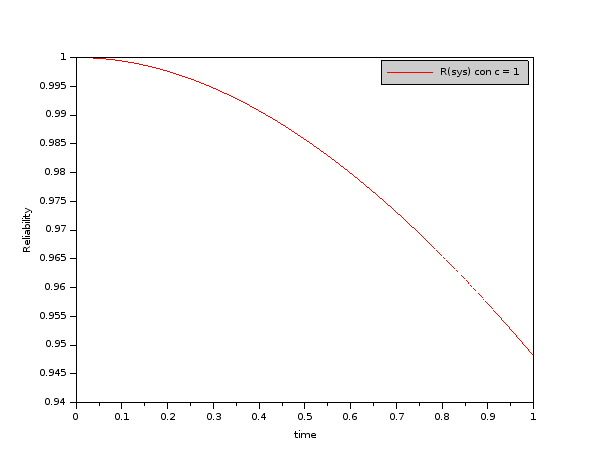
\includegraphics[scale=0.5]{images/Capitulo4/Reliability_BinaryTree.png}
  \caption{Confiabilidad con respecto al tiempo de árbol binario de 4 niveles}  
\label{fig:Reliability_binary_tree_4_levels_2} 
\end{figure}

La cantidad de niveles que se eligió para esta topología depende del número de subsistemas que se requieren.

Los nodos back up se mantienen inactivos, es decir no participan en el procesamiento durante la vida normal del sistema. En caso de producirse una falla, se supone que estos nodos de redundancia, comienzan a funcionar automáticamente, sin ninún tipo de retraso. Esto, que no corresponde con la realidad, permite simplificar los cálculos para este trabajo de tesis.

\subsection{Red distribuida}
El estudio de una topología de red distribuída no es tan sencilla como la que se plantea para un árbol binario. Para el desarrollo de esta red, además de los 6 nodos que representa cada uno de los subsistemas requeridos, se agrega 2 nodos de redundancia. Por lo tanto se tiene una red de 8 nodos. Siguiendo la metodología de desarrollo presentado por \cite{Pradhan82} se llevó a cabo la red que se presenta en la Figura \ref{fig:distributed_net}. 

\begin{figure}[h]
 \centering
 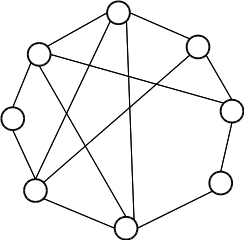
\includegraphics[scale=0.75]{images/Capitulo4/distributed_network.jpg}
  \caption{Red distribuida}  
\label{fig:distributed_net} 
\end{figure}

Esta cuenta con 4 nodos de grado 4, 2 nodos de grado 3, y 2 nodos de grado 2. Ante cualquier falla de alguno de los nodos de la red, esta topología tiene la capacidad formar subredes, que mantien todos los nodos conectados (a excepción del fallado), asegurandose la funcionalidad y reconfiguración del sistema completo. Estratégicamente y para lograr la condición mencionada anteriormente, se crea la \textbf{condición} de que pueden fallar hasta 4 nodos simultaneamento. Esto aseguraría de que la red continuará funcionando aún en la presencia de fallas (tolerante a fallas).

Se modificó la fórmula desarrollada  por \cite{Stivaros92}, para lograr una cohrencia de los modelos que se vienen planteand en el presente trabajo. Teniendo en cuenta que la confiabilidad del sistema completa es: $$R(t) = \prod_{v \in S} e^{- \lambda t}$$

donde $v$ representa el nodo y $S$ es el subsistema funcional. Es decir, que este modelo recorre todos los nodos funcionales. Cuando existen nodos con fallas, y que dejan de ser funcionales, el modelos es el siguiente: $$R_{sys} =\sum_{i=0}^{k} (( \prod_{v \in S} R(t)) - (\prod_{v \notin S} (1 -  R(t) c )))$$

donde c se definió como una \textit{constante de degradación del sistema} para modelar una degradació del sistema.

En la Figura \ref{fig:reliability_distributedNet} se puede observar la \textit{curva de confiabilidad} del sistema, para el caso en el que todos los nodos se encuentran funcionales. 

\begin{figure}[H]
 \centering
 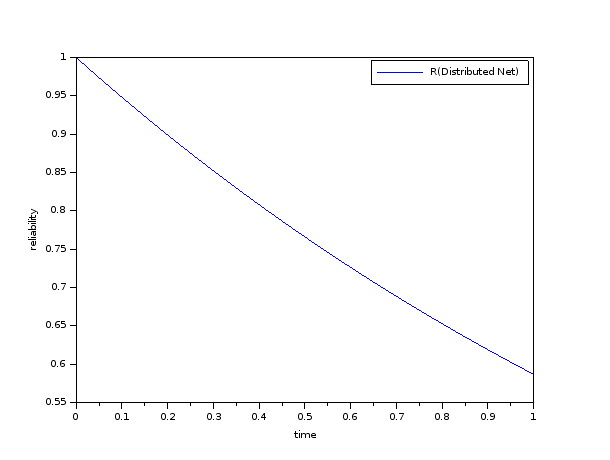
\includegraphics[scale=0.5]{images/Capitulo4/Reliability_DistributedNet.png}
  \caption{Red distribuida}  
\label{fig:reliability_distributedNet} 
\end{figure}


Para el caso de la falla de todos los nodos la \textit{curva de confiabilidad} (Figura \ref{fig:reliability_distributedNet_4Nodes_Fail}) muestra correctamente la degradación esperada de la confiabilidad, con respecto al sistema funcionando correctamente sin ninguna falla.

\begin{figure}[H]
 \centering
 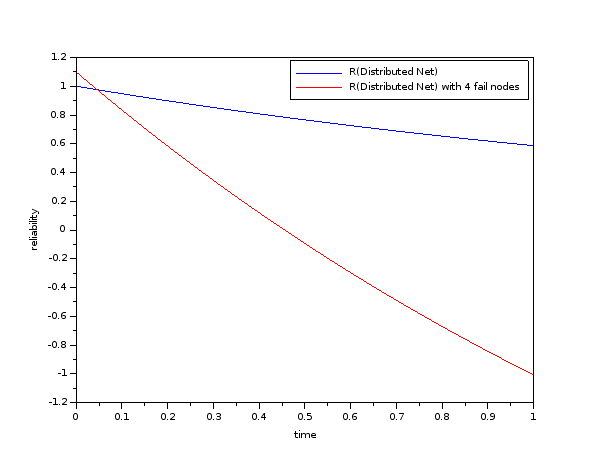
\includegraphics[scale=0.5]{images/Capitulo4/Reliability_DistributedNet_4Nodes_Fail_2.png}
  \caption{Red distribuida}  
\label{fig:reliability_distributedNet_4Nodes_Fail} 
\end{figure}

\subsection{Red hypercube}
Para el caso de la red hypercube se llevaron a cabo modificaciones al modelo planteado por \cite{Mostafa14}, con el propósito de mantener coherencia en los modelos y cálculos que se realizan en este trabajó. Se diseñó una red 3-dimensional, con 8 nodos,  de los cuales 6 nodos corresponden a los diferentes subsistemas y 2 nodos son utilizados de redundancia (Figura \ref{fig:Reliability_Hypercube}).

\begin{figure}[H]
 \centering
 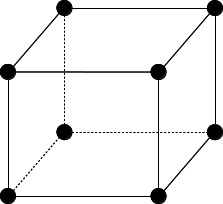
\includegraphics[scale=0.75]{images/Capitulo4/Hypercube2.jpg}
  \caption{Red distribuida}  
\label{fig:Hypercube} 
\end{figure}

En este trabajo de tesis, la confiabilidad se calculó por medio del siguiente modelo: $$R_{sys} = 1- [N (1 - e^{- \lambda t}]$$

Como se puede observar el modelo es similar al modelo de árboles binario. Como se pudo estudiar en la bibliografía, árboles binarios y redes hypercube presentan varias similitudes, incluso se emebebe árboles binarios en este tipo de red. La \textit{curva de confiabilidad} de esta red se la puede observar en la fgura 

\begin{figure}[H]
 \centering
 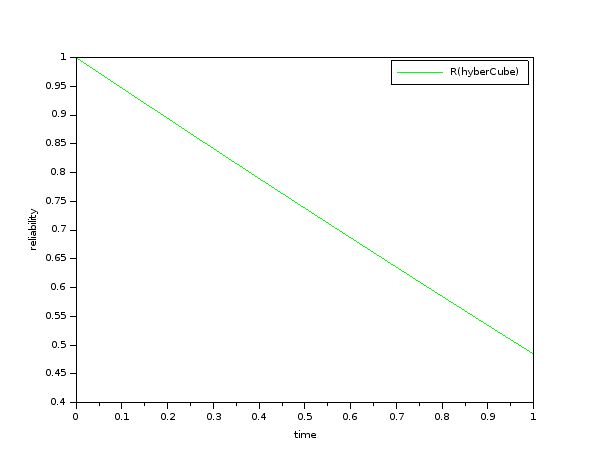
\includegraphics[scale=0.5]{images/Capitulo4/Reliability_Hypercube.png}
  \caption{Red distribuida}  
\label{fig:Reliability_Hypercube} 
\end{figure}

\section{Topología utilizada en la arquitectura a diseñar}

Teniendo en cuenta los modelos presentados anteriormente, se procede a realizar una comparación de las diferentes curvas. El resultado de esto, permitiré conocer de manera analítica qué topología presenta una mayor tolerancia a fallas a travez del tiempo. Además, teniendo en cuenta lo estudiado en el estado de la cuestión, se puede realizar una comparación conceptual de las tres topologías.

La aplicación de árboles binario podríar resultar una buena opción, ya que representa un desarrollo sencillo. En contraposición se puede indicar que existe un alto grado riesgo de que se produzca una falla en el nodo raíz y de su redundancia, lo cual pondría en peligro la misión. Así mismo, presenta otro punto negativo que se puede mencionar y es la gran cantidad de enlaces que esta necesita para mantener a todos los nodos de la red conectados.

Por otra parte, la red distribuída cuenta con la capacidad de distribuir el trabajo en todos sus nodos. Esto quiere decir, que si se produce una falla irrecuperable en cualquiera de sus nodos, la arquitectura podría continuar funcionando sin verse afectada por la ausencia de dicho nodo. Esto demanda un procesamiento computacional extra, y la necesidad de desarrollar algorimtos de ruteo especiales. Además, como punto negativo se puede mencionar que también, al igual que los árboles binarios, necesitan una gran cantidad de enlaces.

Por último, las topologías hypercube tiene un excelente respaldo teórico, exigen menor cantidad de enlaces, y pueden tolerar la falla de una gran cantidad de nodos (hasta el 50\% de los nodos). Su complejidad aumenta en gran medida, cuando se desarrollan arquitecturas de más dimensiones, sin embargo, esto aumenta su confiabilidad.

Como se mencionó en el primer párrafo, se realizó una comparación de módelos de confiabilidad de las tres topologías estudiadas. Se asumió que la distribución de la confiabilidad es exponencial, con una tasa de falla fija de 1/15, y se estudió su evolución en un rango $[0,1]t$. El resultado de esta comparación se la puede observar en la Figura \ref{fig:comparative_reliablities} y en la Tabla \ref{table_comprative_reliability}.

Se observa que tanto las redes distribuidas como la hypercube presenta una mayor confiabilidad a través del tiempo que  los árboles binarios. Si bien, las redes distribuidas y la hypercube tienen una curva similar, la primera presenta una mayor confiabilidad sostenida en el tiempo.

\begin{figure}[H]
 \centering
 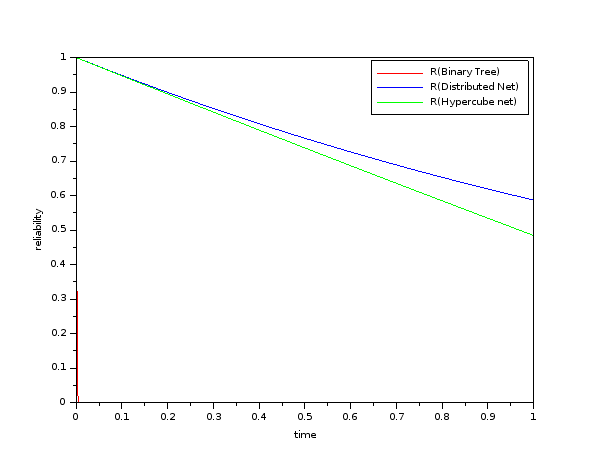
\includegraphics[scale=0.5]{images/Capitulo4/comparative_reliablities.png}
  \caption{Red distribuida}  
\label{fig:comparative_reliablities} 
\end{figure}

\begin{table}[H]
\centering
\caption{Comparación de confiabilidad de topologías}
\label{table_comprative_reliability}
\begin{tabular}{r|r|r|r|}
\cline{2-4}
\multicolumn{1}{l|}{} & \multicolumn{3}{c|}{Topologías de red} \\ \hline
\multicolumn{1}{|c|}{T} & \multicolumn{1}{c|}{Tree Net} & \multicolumn{1}{c|}{Distr Net} & \multicolumn{1}{c|}{Hyper Net} \\ \hline
\multicolumn{1}{|r|}{0} & 1 & 1 & 1 \\ \hline
\multicolumn{1}{|r|}{0.001} & 0.803766 & 0.999947 & 0.999947 \\ \hline
\multicolumn{1}{|r|}{0.002} & 0.64604 & 0.999893 & 0.999893 \\ \hline
\multicolumn{1}{|r|}{0.003} & 0.519265 & 0.99984 & 0.99984 \\ \hline
\multicolumn{1}{|r|}{0.004} & 0.417368 & 0.999787 & 0.999787 \\ \hline
\multicolumn{1}{|r|}{0.005} & 0.335466 & 0.999733 & 0.999733 \\ \hline
\multicolumn{1}{|r|}{...} & ... & ... & ... \\ \hline
\multicolumn{1}{|r|}{0.995} & 0 & 0.948317 & 0.947109 \\ \hline
\multicolumn{1}{|r|}{0.996} & 0 & 0.948266 & 0.947056 \\ \hline
\multicolumn{1}{|r|}{0.997} & 0 & 0.948216 & 0.947003 \\ \hline
\multicolumn{1}{|r|}{0.998} & 0 & 0.948165 & 0.94695 \\ \hline
\multicolumn{1}{|r|}{0.999} & 0 & 0.948115 & 0.946897 \\ \hline
\end{tabular}
\end{table}


Con esto se puede concluir que la topología que presenta un mayor grado de confiabilidad es la que responde a una filosofía distribuida (bajo las condiciones en las que fueron estudiadas). Por lo tanto, la arquitectura satelital, tolerante a fallas y basada en componentes COTS que se desarrolla en la presenta tesis se basa en una \textbf{topología distribuída} para interconectar los diferentes subsistemas. 

\section{Topología propuesta}
Sobre la base de los resultados presentados en \citep{Arias17} se puede establecer que la topoloǵia propuesta es la más adecuada para el desarrollo de una arquitectura tolerante a fallas como se presenta en la Figura \ref{fig:topo_propuesta}. En esta se puede observar que cada subsitema (térmico, power, telemetría, etc.) tiene su propia CPU controladora. Estas CPU se conectan a los nodos. 

\begin{figure}[h]
 \centering
 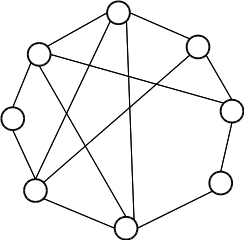
\includegraphics[scale=0.75]{images/Capitulo4/distributed_network.jpg}
  \caption{Red distribuida}  
\label{fig:topo_propuesta} 
\end{figure}

El modelo exige como requerimiento que cada nodo debe estar compuesto por una computadora (componente COTS) que es la encargada de realizar el procesamiento de las tareas. También, debe exitir un puente de comunicación entre la red y la CPU del subsistema. De este modo se hace frente a posibles fallas en la computadora del nodo. Esta conexión se observa en la Figura \ref{fig:conn_prop}

\begin{figure}[h]
 \centering
 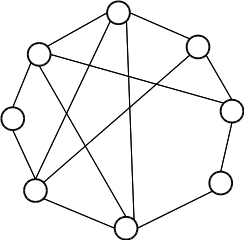
\includegraphics[scale=0.75]{images/Capitulo4/distributed_network.jpg}
 \caption{Red distribuida}  
\label{fig:conn_prop} 
\end{figure}




% section that talk about the comm protocol
\section{Protocolo de comunicación}
Como se estudió en el marco teórico, en una arquitectura
de comunicación, el protocolo CAN trabaja en las
capas inferiores del modelo de OSI. CAN propone cómo debe ser
el medio físico, y la manera de transmisión de las señales.
Además, preve cuál es la estrategia a utilizar  para sincronizar
la transmisión de datos sin nigún tipo de latencia, ni tampoco
colisiones de mensajes. Así, este protocolo permite que estos
sean envíados teniendo en cuenta sus prioridades, eliminando las colisiones, y
por lo tanto también, el tiempo de espera en la que los nodos se quedan
relegados cuando han tratado de enviar un mensaje al mismo tiempo.

Este protocolo no establece nada sobre ruteos de mensajes, tipos de mensajes y
tipos de datos, que a la hora de desarrollar una arquitectura de aviónica es
importante tener en cuenta esos detalles. Es necesario, que exista una
capa de servicios que facilite la comunicación entre aplicaciones de usuarios
de diferentes nodos, y la comunicción entre las aplicaciones de usuario
y el protocolo CAN (de bajo nivel) en sí.
Además, teniendo en cuenta los resultados obtenidos en las secciones
anteriores, se necesita además, diseñar un protocolo de comunicación
basado en redes distribuidos, y que a su vez, esté basado en CAN.

Por tales motivos, surge la necesidad
de diseñar un protocolo de comunicación basado en CAN, que se ``monte'' sobre
las capas superiores del modelo de referencia de OSI; y que permita
la distribución de las tareas y el procesamiento llevado a cabo
por los nodos. 

El protocolo CANae se encuentra en su primera versión 0.1 Alpha. Esto hace
referencia a que en esta instancia de trabajo se tratar de comprender
el problema y llevar a cabo un diseño preliminar de protocolo. De esta
manera se podrá extraer, tanto puntos positivos, como puntos negativos; o
más bien fortalezas y debilidades del stack de servicios que brinda CANae.

CANae actúa en la capa de aplicación del modelo de referencia de OSI. CANae
divide esta capa en dos subcapas:
\begin{itemize}
\item CANae Application Layer
\item CANae High Application layer
\end{itemize}

\begin{figure}[h!]
 \centering
 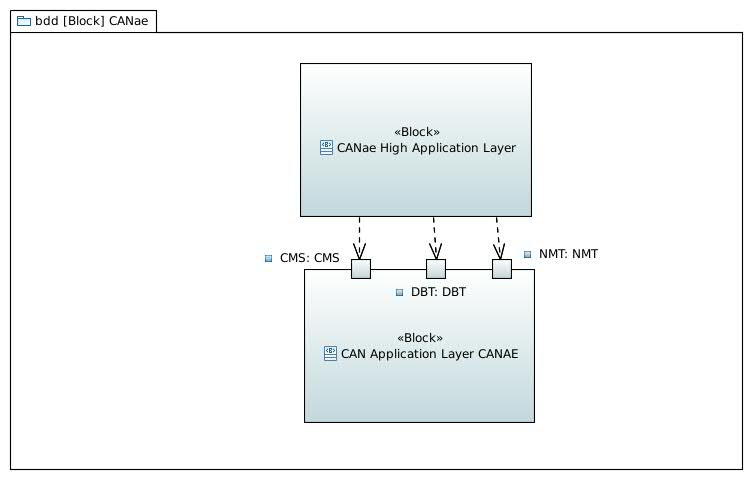
\includegraphics[scale=0.5]{images/Secciones/AppendixA/CANAE.JPG}
  \caption{Estructura de la capa de aplicación de CANae en alto nivel}
\label{fig:CANAEC4}
\end{figure}

Esto puede observar se en la Figura \ref{CANAEC4}. En el gráfico se observa que
la CANae application Layer, cuenta con 3 interfaces:n
\begin{itemize}
\item \textbf{CMS}: ofrece un ambiente orientado a objecto para diseñar aplica-
ciones de usuario. Esta entidad ofrece variables y eventos, y específica como un módulo pude acceder a
las interfaces de CAN.
\item \textbf{NMT}: ofrece un ambiente orientado a objetos para permitir que un módulo (el
NMT Master) se ocupe de la inicialización y posibles fallas de otros módulos (NMT Slaves).
\item \textbf{DBT}: ofrece el servicio para distribuir dinámicamente el identificador de para los diferentes nodos.
\end{itemize}
Debe destacarse que, el servicio CMS ofrece un ambiente orientado a objeto  para diseñar
aplicaciones de usuario, es decir, que ofrece la posibilidad de modelar el
comportamiento del sistema en forma de objeto. Este servicio ofrece la posibilidad
de crear variables y eventos, según las necesidades de los usuariosm que son
utilizadas para diseñar y especificar como la funcionalidad de un módulo puede
acceder a las interfaces de bajo nivel de CAN. Esto propone un grado de innovación
al tratar al protocolo, a los datos, mensajes y eventos como objetos, permitiendo así
un modelado orientado a objetos. Por tal motivo, este protocolo fue modelado
con SysML (System Modeling Language).
Para mayor detalle de estas interfaces se debe consultar en el apéndice \ref{Appendix:A}.

Agregando, dentro de esta capa existen dos entidades que juegan un papel importante
(consultar apéndice \ref{Appendix:A}) las cuales son:
\begin{itemize}
\item \textbf{Gestor de mensajes}: este se encarga de gestionar los mensajes que son enviados y recibidos desde la red.
Esta entidad debe ser capaz de determinar si el mensajes contiene datos o eventos. Trabaja en conjunto
con el CMS.
\item \textbf{Gestor de nodo}: esta entidad se encarga de llevar el control de los nodos existenten en la red. En este
nodo se encuentra la tabla de ruteo primario y secundario necesarios para la correcta comunicación.
\end{itemize}

La subcapa denominada CAN High Application Layer tiene una función más del lado de la gestión de nodos y tareas.
En esta capa se desarrollan los algoritmos necesarios para realizar el ruteo y la reconfiguración de la red ante
fallas, por lo tanto en la High Application Layer se debe implementar la FDIR. El protocolo no define ninún
algoritmo de ruteo, por lo que queda para el usuario la definición de los algoritmos.
El protocolo  recomienda desarrollar dos algoritmos, el primario y el secundario.
Para aumentar la tolerancia a fallas se pueden desarrollar más algoritmos
secundarios, y el switch entre algoritmos, puede depender de medidas de perfomance.

Así, queda conformada el protocolo de comunicación CANae como uno de los
principales productos de este trabajo de tesis. 


\vspace{1cm}
\noindent\rule{\textwidth}{2pt}

\textbf{\Large{Resúmen}}

En este capítulo se llevó a cabo un estudio de tres tipos de topologías tolerantes
a fallas que fueron candidatas a ser utilizadas como base en la
arquitectura que se diseñó en este trabajo de tesis. 

Teniendo en cuenta los modelos que se han desarrollado en este capítulo se compararon las diferentes curvas de confiabilidad. El resultado de esto, permitió conocer de manera analítica qué topología presenta una mayor tolerancia a fallas a través del tiempo.

Se asumió que la distribución de la confiabilidad es exponencial, con una tasa de falla fija de 1/15, y se estudió su evolución en un rango $[0,1]t$. El resultado de esta comparación se la puede observar en la Figura \ref{fig:comparative_reliablities} y en la Tabla \ref{table_comprative_reliability}.

Se observa que tanto las redes distribuidas como la hypercube presentan una mayor confiabilidad a través del tiempo que  los árboles binarios. Si bien, las redes distribuidas y la hypercube tienen una curva similar, la primera presenta una mayor confiabilidad sostenida en el tiempo.

Así en este capítulo se llegó a la conclusión de que la topología que presenta un mayor grado de
confiabilidad es la que responde a una filosofía distribuida.  Por lo tanto, la arquitectura satelital, tolerante a fallas y basada en componentes COTS que se desarrolla en la presenta tesis se basa en una \textbf{topología distribuida} para interconectar los diferentes subsistemas.
